% ****** Start of file apssamp.tex ******
%
%   This file is part of the APS files in the REVTeX 4.1 distribution.
%   Version 4.1r of REVTeX, August 2010
%
%   Copyright (c) 2009, 2010 The American Physical Society.
%
%   See the REVTeX 4 README file for restrictions and more information.
%
% TeX'ing this file requires that you have AMS-LaTeX 2.0 installed
% as well as the rest of the prerequisites for REVTeX 4.1
%
% See the REVTeX 4 README file
% It also requires running BibTeX. The commands are as follows:
%
%  1)  latex apssamp.tex
%  2)  bibtex apssamp
%  3)  latex apssamp.tex
%  4)  latex apssamp.tex
%
\documentclass[%
reprint,
%superscriptaddress,
%groupedaddress,
%unsortedaddress,
%runinaddress,
%frontmatterverbose, 
%preprint,
%showpacs,preprintnumbers,
%nofootinbib,
%nobibnotes,
%bibnotes,
amsmath,amssymb,
aps,
%pra,
%prb,
%rmp,
%prstab,
%prstper,
%floatfix,
]{revtex4-1}

\usepackage{graphicx}% Include figure files
\usepackage{dcolumn}% Align table columns on decimal point
\usepackage{bm}% bold math
\usepackage{hyperref}% add hypertext capabilities
\usepackage[mathlines]{lineno}% Enable numbering of text and display math
\usepackage{amsmath} % assumes amsmath package installed
\usepackage{amssymb}  % assumes amsmath package installed

\usepackage{epsfig} % for postscript graphics files
\documentclass[12pt,twoside,a4paper]{report}

\setlength{\headheight}{26pt}
\usepackage{mathptmx} % assumes new font selection scheme installed
\usepackage{times} % assumes new font selection scheme installed

%\linenumbers\relax % Commence numbering lines

%\usepackage[showframe,%Uncomment any one of the following lines to test 
%%scale=0.7, marginratio={1:1, 2:3}, ignoreall,% default settings
%%text={7in,10in},centering,
%%margin=1.5in,
%%total={6.5in,8.75in}, top=1.2in, left=0.9in, includefoot,
%%height=10in,a5paper,hmargin={3cm,0.8in},
%]{geometry}
\def\bibsection{\section{Bibliography}} 
\begin{document}
	
	\preprint{APS/123-QED}
	
	\title{Optical and Transport properties of semiconductors heterostructures}% Force line breaks with \\
	
	\author{Diego Oliveira}
	\affiliation {Instituto de Física, Universidade Estadual de Campinas-Unicamp, Campinas, São Paulo, 13083-859, Brazil}
	\email{dso@ifi.unicamp.br}
	
	\date{\today}% It is always \today, today,
	%  but any date may be explicitly specified
	
	\begin{abstract}
	In this paper we review the optical and transport properties of semiconductors heterostructures. Transport properties as the drift-diffusion equation, the diffusion current, the thermionic emission current, and tunelling current. Optical properties of the complex refractive index, the absorption coefficient, the phenomena of reflection, transmission, and the different absorption processes.
		
		\begin{description}
			\item[PACS numbers]
			73.40.-c, 73.21.Fg, 78.20.Ci.
		\end{description}
	\end{abstract}
	
	\pacs{Valid PACS appear here}% PACS, the Physics and Astronomy
	% Classification Scheme.
	\keywords{Semiconductor lasers, quantum wells}%Use showkeys class option if keyword
	%display desired
\maketitle
\renewcommand{\thesection}{\arabic{section}}
\renewcommand{\thesubsection}{\thesection.\arabic{subsection}}
\renewcommand{\thesubsubsection}{\thesubsection.\arabic{subsubsection}}

% Fix references
\makeatletter
\renewcommand{\p@subsection}{}
\renewcommand{\p@subsubsection}{}
\makeatother
	%\tableofcontents
	
\section{INTRODUCTION}
The junctions formed between two semiconductors(Fig \ref{structure}a) with different energy gaps are referred to as heterojunction. In general, heterostructures offer a wide range of design choices for novel semiconductor devices (e.g., diodes, transistors, and optoelectronic devices). In an ideal heterojunction, the interface is atomically abrupt (In practical cases, such an ideal structure is nearly realized in $ Al_xGa_{1-x}As/GaAs $ heterojunctions). The main advantages are related to the control of the charge carrier transport by controlling the energy barriers and potential variations (on a quantum level, Fig.\ref{structure}b) and to the ability of heterostructures to confine the optical radiation (which is especially essential in optoelectronic devices). Heterostructures are normaly grown by either metal-organic chemical vapor deposition (MOCVD) or molecular beam epitaxy (MBE) epitaxial techniques \cite{yacobi}. 


\begin{figure}[!h]
	\centering
	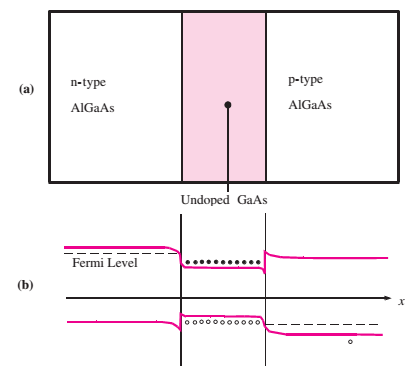
\includegraphics[scale=0.81]{STRUCTURE.png}
	\caption{(a) Structure of a double heterojunction. (b) Dependence of the band
		edge energies along the growth direction x \cite{yuyu}.
		%\caption{Hypothetical absorption spectrum for a typical semiconductor as a function of photon energy
		\label{structure}}
\end{figure}


	
	
\section{TRANSPORT PROPERTIES}
A good understanding of charge carrier transport and electrical conduction is essential for selecting or developing electronic materials for device applications. 
	
\subsection{Drift-Diffusion Equation}

The drift-diffusion model may be obtained by taking zeroth order moments of the  Boltzmann Transport Equation and adjoining the Poisson equation. Thus, one obtains the system for N carriers with concentration $ n_i $, carrier recombination $ R_i $, current density $ J_i $ , (signed) charge $ e_i $, i = 1,..., N:
	
\begin{equation}
		e_i\dfrac{\partial n_i }{\partial t} + \nabla \cdot	  J_i = -e_i R_i
\end{equation}
\begin{equation}
		E =- \nabla\phi
\end{equation}
\begin{equation}
	\nabla \cdot(\epsilon\nabla\phi) = -\sum e_i n_i - k_1
\end{equation}
Here the dielectric constant is denoted by $ \epsilon $, $ k_1 $ is the net impurity concentration, and $ \phi $ is the electrostatic potential. There still remains the issue of determining the constitutive current relations. Classical drift-diffusion theory gives, for N = 2, $ n_l  = n$ (the electron density) , and $ n_2  = p$ (the hole density),
	
\begin{equation}
	J_n =-e \mu_n n E + eD_n \dfrac{dn}{dx}
		\label{dde}
\end{equation}
\begin{equation}
		J_p =-e \mu_p p E -  eD_p \dfrac{dp}{dx}
		\label{dde2}
\end{equation}
	
The electronic charge modulus $ e $ is positive here, and $ n $ and $ p $ denote the electron and hole densities, respectively. The use of the Einstein relations linking the mobilities, $ \mu_n $, $ \mu_p $, and the diffusion coefficients, $ D_n $, $ D_p $, is common. These relations are specified by
	
\begin{equation}
		D_n = (kT/e)\mu_n
\end{equation}
\begin{equation}
		D_p = (kT/e)\mu_p
\end{equation}
	
The heterostructure drift-diffusion Eq.\ref{dde} and Eq.\ref{dde2} may be solved analytically for the case of steady-state transport in one dimension, provided that recombination and generation may be neglected. The equations and their solutions can be incorporated into the conventional pn junction theory to obtain expressions for the $ I(V ) $ characteristics of a heterojunction.
	
	\subsection{Transport Carriers Mechanisms}
	The current across heterostructure junction is mainly due to majority carriers, by three distinct mechanisms: \textbf{diffusion} of carriers, \textbf{thermionic emission} of carriers and \textbf{quantum-mechanical tunneling}. The diffusion theory assumes that the driving force is distributed over the length of the depletion layer. The thermionic emission theory on the other hand postulates that only energetic carriers, those, which have an energy equal to or larger than the conduction band, contribute to the current flow. Quantum-mechanical tunneling through the barrier takes into account the wave-nature of the electrons, allowing them to penetrate through thin barriers. In a given junction, a combination of all three mechanisms could exist. However, typically one finds that only one current mechanism dominates.
	The analysis reveals that the diffusion and thermionic emission currents can be written in the following form:
	
	\begin{equation}
	J_n = evN_c exp({-\frac{\phi_B}{V_t}})[exp(\frac{V_a}{V_t}) - 1]
	\end{equation}
	
	This expression states that the current is the product of the electronic charge $ e $, a velocity $  v $, and the density of available carriers in the semiconductor located next to the interface, where $ V_a $ is the applied voltage, $ \phi_B $ the Schottky barrier height and $ N_c $ is the effective density of states. The velocity equals the mobility multiplied by the field at the interface for the diffusion current and the Richardson velocity for the thermionic emission current. The minus one term ensures that the current is zero if no voltage is applied as in thermal equilibrium any motion of carriers is balanced by a motion of carriers in the opposite direction.
	
	
	\subsection*{Diffusion Current}
	
	Assuming that the depletion layer is large compared to the mean free path, so that the concepts of drift and diffusion are valid. The resulting current density equals:
	
	\begin{equation}
	J_n = e\mu_n E_{max }N_c exp({-\frac{\phi_B}{V_t}})[exp(\frac{V_a}{V_t}) - 1]
	\end{equation}	
	
	where $ E_{max} $ is electric field at the heterostructure interface. So that the prefactor equals the drift current at the heterostructure interface, which for zero applied voltage ($ V_a $) exactly balances the diffusion current.
	
	\subsection*{Thermionic Emission Current}
	The thermionic emission theory assumes that electrons, with an energy larger than the top of the barrier, will cross the barrier provided they move towards the barrier. So the  current can be expressed as:
	
	\begin{equation}
	J_{MS} = A^* T^2 exp({-\frac{\phi_B}{V_t}})[exp(\frac{V_a}{V_t}) - 1]
	\end{equation}	
	where $ A^* $ is the Richardson constant and $ \phi_B $ is the Schottky barrier height. The expression for the current due to thermionic emission can also be written as a function of the average velocity with which the electrons at the interface approach the barrier. This velocity is referred to as the Richardson velocity $ v_R = \sqrt{\frac{kT}{2\pi m}} $, so that the current density becomes:	
	
	\begin{equation}
		J_n = ev_R N_c exp({-\frac{\phi_B}{V_t}})[exp(\frac{V_a}{V_t}) - 1]
	\end{equation}
	
	\subsection*{Tunneling Current}
The tunneling current is obtained from the product of the carrier charge, velocity and density. The velocity equals the
Richardson velocity, the velocity with which on average the carriers approach the barrier. The carrier density equals the
density of available electrons, n, multiplied with the tunneling probability, $ \Theta $, yielding
	
	\begin{equation}
	J_n = e n v_R \Theta
	\end{equation}
	
The tunneling probability term $ \Theta $, is added since the total current depends on the carrier flux arriving at the tunnel barrier multiplied with the probability $ \Theta $, that they tunnel through the barrier.  The tunneling probability is obtained from:

\begin{equation}
\Theta = exp (-\frac{4}{3}\frac{\sqrt{2em^*}}{\hbar} \frac{{\phi_B}^{3/2} }{E})
\end{equation}
	
	
	
	
	
	\section{OPTICAL PROPERTIES}
	The interaction of light with a semiconductor, allows us to observe the phenomena of \textbf{absorption}, \textbf{reflection} and \textbf{transmission}. From these optical effects, we obtain much of the information we have concerning the energy band structure and electronic precesses in semiconductors. 
	
	
	
	
	\subsection{Complex Refractive Index and Absorption Coefficient}
	
	By means of classical electromagnetic theory we may relate  complex refractive index ($ n^*$) through the complex dielectric function ($ \epsilon^* $) as defined by means of the equation, $ \epsilon^*(\omega)  = \epsilon(\omega) - i\sigma/2\pi v = \epsilon_1(\omega) + i\epsilon_2(\omega) $, where $ \epsilon $ is the ordinaty permittivity and $ \sigma $ the conductivity. The complex refractive index and dielectric function are related by means of the equation:
	
	\begin{equation}
		n^*(\omega) = n(\omega) + ik(\omega)  =  {[\epsilon_1(\omega) + i\epsilon_2(\omega)]}^\frac{1}{2}
		\label{index}
	\end{equation}
	
	From  Eq.\ref{index} it follows that, $ \epsilon_1 = n^2 - k^2$ and $ \epsilon_2 = 2nk $, these quantities are most frequently plotted in order to describe the optical proprieties of a material.
	
	
	The real part of the refractive index $n(\omega)$ determines the propagation velocity.
	The imaginary part $ k(\omega) $ called the extinction coefficient, also called the attenuation index, determines the absorption coefficient:
	
	\begin{equation}
		\alpha = \dfrac{4\pi}{\lambda} k
	\end{equation}
	
	In semiconductors, the absorption coefficient is a strong function of the wavelenght or photon energy. Near the absorption edge, the absorption coefficient can be expressed as
	\begin{equation}
		\alpha \propto (hv - E_{g})^\gamma 
		\label{ab}
	\end{equation}
	where $ hv $ is the photon energy and $ \gamma $ is a constant. There exist two types of band-to-band transitions: allowed and forbidden (forbidden transitions take into accont the small but finite momentum of photons and are much less probable). For direct bandgap materials, transitions mostly occur between two bands of the same k value, as transitions (a) and (b) in Fig.\ref{transitions}. While allowed direct transitions can occour in all $  k $ values, forbidden direct transitions can only occur at $ k \neq 0 $. In the one electron approximation, $ \gamma = 1/2 $ for allowed and $ \gamma = 3/2 $ for forbidden direct transitions. For $ k=0 $ at which the bandgap is defined, only allowed transition occurs and thus it is used in determining the bandgap experimentally. For indirect transitions ((c) in Fig.\ref{transitions}), phonons are involved in order to conserve momentum. In these transitions, phonons (with energy $ E_p $) are either absorbed or emitted, and the absorption coefficient is midified to $ \alpha \propto (hv - E_{g} \pm E_p)^\gamma $ where $ \gamma $ equals 2 and 3 for allowed and forbidden indirect transitions, respectively.
	
	
	
	\begin{figure}[!h]
		\centering
		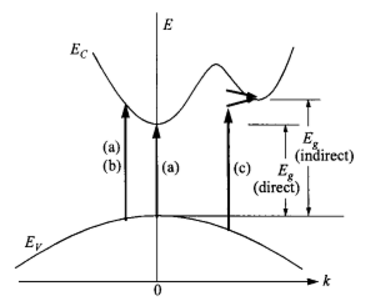
\includegraphics[scale=0.8]{transitions.png}
		\caption{Optical Transitions: (a) allowed and (b) forbiden direct transitions; (c) indirect transition involving phonon emission (upper arrow) and phonon absorption (lower arrow)\cite{sze}.
			\label{transitions}}
	\end{figure}
	
	\subsection{Reflectivity and Transmissivity}
	The reflectivity at the surface of a semi-infinite crystal can be calculated by considering incident and reflected waves in the vacuum and a trasmitted wave in the crystal. By applying electromagnetic boundary conditions at the crystal surface one can obtain an expression for the reflectivity. This expression is somewhat complicated for an arbitrary angle of incidence, so let consider a case of normal incidence. The amplitude of the electric field in the reflected wave, $ E_{ref} = r(\omega)E_{inc} $, where $  r(\omega) $ is give by
	\begin{equation}
		r(\omega) =  \rho(\omega) exp[i\theta(\omega)] = \dfrac{n + ik - 1}{n + ik +1}
	\end{equation}
	where $ \rho(\omega)  $ is the modulus of $ r(\omega) $, and $ \theta(\omega) $ is the phase difference between the electric filds of the reflected and incident waves.
	The experimentally measurable reflectivity, $ R(\omega) $, relates the incident and reflected intensities, $ I_{inc} $ and $ I_{ref} $, $ I_{ref}  = R(\omega)I_{inc}$ where
	\begin{equation}
		R(\omega) =|r(\omega)| ={\rho(\omega)}^2  = \dfrac{(n-1)^2 + k^2}{(n+1)^2 + k^2}
		\label{refre}
	\end{equation}
	and the transmission coefficient for the normal incidence is given by
	\begin{equation}
		T(\omega) = \dfrac{(1 - R^2)exp(-4\pi x/ \lambda)}{1 - R^2exp(-8\pi x/ \lambda)}
	\end{equation}
	where $ x $ is the thickness of the sample.
	
	When light passes through a semiconductor, absorption of light and generation of electron-hole pairs occur, and the light intensity $  P_{op} $ diminishes with distance, $ d P_{op}(r)/dr = - \alpha P_{op}(r)$, the solution of this expression gives an exponential decay of intensity, $ P_{op}(r) =P_0 (1-R)exp(- \alpha r)$, where $ P_0 $ is the external incident light intensity and R is the reflection (Eq.\ref{refre}).
	
	In a semiconductor sample of thickness $ x $ where the product $ \alpha x $ is not large, multiple reflections will occur between the two interfaces. Summing up all the light components in the backward direction, the total reflection coefficient is calculed to be:
	
	\begin{equation}
		R_t = R[1 + \dfrac{(1 - R^2)exp(-2\alpha x)}{1 - R^2exp(-2\alpha x)}]
		\label{refre}
	\end{equation}
	and the transmission coefficient for the normal incidence is given by
	\begin{equation}
		T_t = \dfrac{(1 - R^2)exp(-2\alpha x)}{1 - R^2exp(-2\alpha x)}
	\end{equation}
	where $ x $ is the thickness of the sample.
	
	By analyzing the $ R_t - \lambda $ or $ T_t - \lambda $ data at normal incidence, or by making observations of $ R_t $ or $ T_t $ for different angles of incidence, both $ n^* $ and $ k $ can be obtained and related to transitions energy between bands.
	
	\subsection{Optical Absorption}
	
	A typical relationship between the absorption coefficient and the photon energy observed in a crystalline semiconductor is shown in Fig.\ref{spectrum}, where various possible absorption processes are illustrated. Some of this processes will be discussed in the next topics.
	%In Fig.(\ref{spectrum}) we can see some processes that can contribute to the absorption, some of this processes will be discussed in the next topics.
	\begin{figure}[!h]
		\centering
		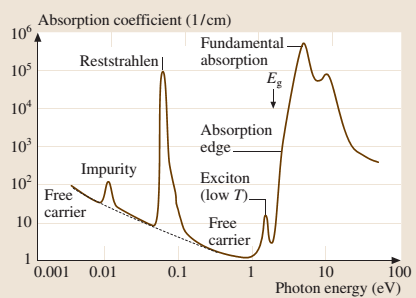
\includegraphics[scale=0.6]{Spectrumm.png}
		\caption{Absorption coefficient plotted as a function of
			the photon energy in a typical semiconductor, illustrating
			various possible absorption processes \cite{ch3}.
			%\caption{Hypothetical absorption spectrum for a typical semiconductor as a function of photon energy
			\label{spectrum}}
	\end{figure}
	
	\subsection*{Exciton Absorption}
	As indicated in Fig.\ref{spectrum}, some structure in the absorption spectra of semiconductors is often observed just below the fundamental absorption edge. This structure is due to exciton absorption. The energy band approximation for one electron, where the rest of the crystal was treated as a periodic potential, in this case there are no allowed energy states between the minima of the conduction bands and the maxima of the valence bands. When a electron-hole pair is created by absorption of a photon inside a semiconductor, the pair experiences an attractive Coulomb force. The latter is responsible for the creation of a bound state called an exciton. The appropriate modification of Eq.\ref{ab} for exciton absorption (allowed direct transition) is $  \alpha \propto (hv - E_{g} - E_{xn})^{1/2 } $ where $ E_{xn} $ is the exciton energy.
	
	\subsection*{Free Carrier Absorption}
	
	When the energy of the incident radiation is too small to create electron-hole pairs or excitons, other absorption processes can occur. The absorption of radiation by electrons in the conduction bands or by holes in the valence bands produces an absorption background below the fundamental absorption edge which increases with wavelength as indicated in Fig.\ref{spectrum}. In this process the electric fild of the incident radiation accelerates the free carries, which, in turn are decelerated by collisions with the lattice. Thus the energy is converted to heat.
	
	
    \subsection*{Lattice Absorption}
	
	Fig.\ref{spectrum} shows an absorption band due to optical phonons which is almost as strong as absorption due to electron transitions from the valence to conduction bands. This absorption is due to electric dipole coupling between photons and phonons which arises from the motion of charged atoms in the crystal (the structure on the high-energy side is due to multiple phonon absorption). Thus this absorption is strong for semiconductors with an ionic component of bonding and weak for those with ourely covalent bonding. If the radiation from a hot body is reflected several times from an ionic crystal, the dominant remaining frequencies will be those in this band of energy. For this reason this absorption is called the "restrahlen" or "residual ray" band.
	
	
	
	
	%Since the photon is a transverse electromagnetic wave, it couples most strongly to the transverse optical phonons. For photon frequencies between the transverse and longitudinal optical phonon frequencies, the reflection is very high. 
	
	
	
\subsection*{Impurity Absorption}
	This absorption process is that due to direct band-to-impurity transition. The transition probability has the same form as for direct band-to-band transitions.
	
\section*{ACKNOWLEDGMENT}
		
The author thanks CAPES for the financial support and Unicamp for providing the infrastructure for this research.

\begin{thebibliography}{10}
		\thispagestyle{empty} % retirar a numeração desta página.
	\bibitem{yuyu}
	P. Y. Yu,
	\newblock \textit{"Fundamentals of Semiconductors".}
	\newblock Springer-Verlag US (2010). 

\bibitem{yacobi}
B. G. Yacobi,
\newblock \textit{"Semiconductor Materials An Introduction to Basic Principles".}
\newblock Kluwer Academic Publishers (2004). 


\bibitem{sharma}
B. L. Sharma, R. K. Purohit and B. R. Pamplin, 
\newblock \textit{"Semiconductor Heterojunctions".}
\newblock Pergamon Press (1974).

\bibitem{wolfe}
C. M. Wolfe, N. Holonyak and G. E. Stillman,
\newblock \textit{ "Physical Properties of Semiconductors".}
\newblock Prentice-Hall International Editions (1989).


\bibitem{sze}
S. M. Sze,
\newblock \textit{"Physics of Semiconductor Devices".}
\newblock Wiley-Interscience (1969).


\bibitem{gaas}
J. G. Ruch and G. S. Kino,
\newblock \textit{ "Transport Properties of GaAs".}
\newblock Phys Rev. 174(3), 921 (1968).

\bibitem{gaas}
K. B. Wong, M. Jaros, I. Morrison, and J. P. Hagon,
\newblock \textit{ "Electronic Structure and Optical Properties of Si-Ge Superlattices".}
\newblock Phys. Rev. Lett. 60(21), 2221 (1988).



\bibitem{ch3}
A. Willoughby, P. Capper and S. Kasap,
\newblock \textit{"Springer Handbook of Electronic and Photonic Materials".}
\newblock Springer-Verlag US (2007). 






	
\end{thebibliography}
	

	
	
	
	%%%%%%%%%%%%%%%%%%%%%%%%%%%%%%%%%%%%%%%%%%%%%%%%%%%%%%%%%%%%%%%%%%%%%%%%%%%%%%%%
	
	
	
	
	
	
	
	
	
	
\end{document}
%
% ****** End of file apssamp.tex ******
